%\begin{tikzpicture}
%	\pgfplotsset{ticks=none}
%    \begin{axis}[
%            xmin=-3,xmax=3,
%            ymin=-3,ymax=3,
%            zmin=-2,zmax=2,
%            xlabel={$x$},
%            ylabel={$y$},
%            zlabel={$z$},
%            zlabel style={rotate=90},
%            view={10}{20},
%            width=3cm,
%            height=3cm]
%        \addplot3[mesh,black,domain=0:2*pi,y domain=0:pi,samples=10,samples y=10]({2*cos(deg(x))*sin(deg(y))},{sin(deg(x))*sin(deg(y))},{cos(deg(y))});
%    \end{axis}
%    
%	\node[text width=1.7cm] at (0.5,-0.4) {$\scriptstyle \frac{x^2}{4}+y^2+z^2=1$};
%\end{tikzpicture}
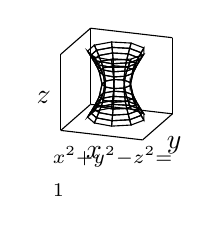
\begin{tikzpicture}
	\pgfplotsset{ticks=none}
    \begin{axis}[
            xmin=-3,xmax=3,
            ymin=-3,ymax=3,
            zmin=-2,zmax=2,
            xlabel={$x$},
            ylabel={$y$},
            zlabel={$z$},
            zlabel style={rotate=90},
            view={20}{20},
            width=3cm,
            height=3cm]
        % x^2+y^2-z^2=1
        \addplot3[mesh,black,domain=1:2,y domain=0:2*pi,samples=6,samples y=10]({x*cos(deg(y))},{x*sin(deg(y))},{sqrt(x^2-1)});
        \addplot3[mesh,black,domain=1:2,y domain=0:2*pi,samples=6,samples y=10]({x*cos(deg(y))},{x*sin(deg(y))},{-sqrt(x^2-1)});
    \end{axis}
    
    \node[text width=1.6cm] at (0.7,-0.4) {$\scriptstyle x^2+y^2-z^2=1$};
\end{tikzpicture}
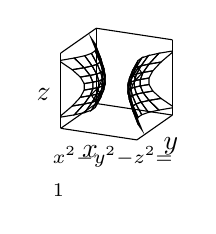
\begin{tikzpicture}
	\pgfplotsset{ticks=none}
    \begin{axis}[
            xmin=-3,xmax=3,
            ymin=-3,ymax=3,
            zmin=-2,zmax=2,
            xlabel={$x$},
            ylabel={$y$},
            zlabel={$z$},
            zlabel style={rotate=90},
            view={25}{20},
            width=3cm,
            height=3cm]
        % x^2-y^2-z^2=1
        \addplot3[mesh,black,domain=-1.2:1.2,y domain=-1.2:1.2,samples=8,samples y=8]({cosh(x)*cosh(y)},{cosh(x)*sinh(y)},{sinh(x)});
        \addplot3[mesh,black,domain=-1.2:1.2,y domain=-1.2:1.2,samples=8,samples y=8]({-cosh(x)*cosh(y)},{cosh(x)*sinh(y)},{sinh(x)});
        
    \end{axis}
    
    \node[text width=1.6cm] at (0.7,-0.4) {$\scriptstyle x^2-y^2-z^2=1$};
\end{tikzpicture}
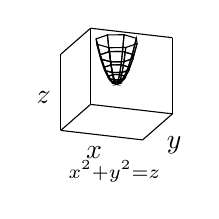
\begin{tikzpicture}
	\pgfplotsset{ticks=none}
    \begin{axis}[
            xmin=-3,xmax=3,
            ymin=-3,ymax=3,
            zmin=-2,zmax=2,
            xlabel={$x$},
            ylabel={$y$},
            zlabel={$z$},
            zlabel style={rotate=90},
            view={20}{20},
            width=3cm,
            height=3cm]
        \addplot3[mesh,black,domain=0:2*pi,y domain=0:1.5,samples=9,samples y=6]({y*cos(deg(x))},{y*sin(deg(x))},{y^2});
        
    \end{axis}
    
    \node[text width=1.2cm] at (0.7,-0.4) {$\scriptstyle x^2+y^2=z$};
\end{tikzpicture}
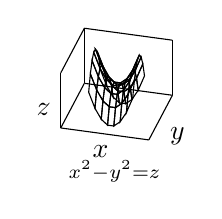
\begin{tikzpicture}
	\pgfplotsset{ticks=none}
    \begin{axis}[
            xmin=-3,xmax=3,
            ymin=-3,ymax=3,
            zmin=-2,zmax=2,
            xlabel={$x$},
            ylabel={$y$},
            zlabel={$z$},
            zlabel style={rotate=90},
            view={15}{40},
            width=3cm,
            height=3cm]
        \addplot3[mesh,black,domain=-1.5:1.5,y domain=-1.5:1.5,samples=8,samples y=8]({x},{y},{x^2-y^2});
        
    \end{axis}
    
    \node[text width=1.2cm] at (0.7,-0.4) {$\scriptstyle x^2-y^2=z$};
\end{tikzpicture}
